\graphicspath{ {06-BLspecScrpts/Figures/} }

\section{Beam-line specification and scripts}

\subsection{Beam-line specification}

The specification is defined in the form of a parameter table.
The table is loaded using a plain text file in CSV format.
An example, specifying the PoPLaR beam line is shown in
table~\ref{Tab:BLspec}.
The simplest way to generate the CSV file is to use Excel to
manipulate one of the examples provided in the \texttt{11-Parameters}
directory of the \texttt{LinearOptics} package.
The parameter table is organised in 8 columns:
\begin{description}
  \item{\texttt{Stage}:} (integer) allows stages in the beam line to
    be defined.
    The number is arbitrary and is used only in the generation of a
    unique name for each element.
    \texttt{Stage} can be defined for clarity in labelling and
    presentation.
  \item{\texttt{Section}:} (string) allows sections in the beam line
    to be distinguished.
    As in the case of \texttt{Stage}, \texttt{Section} may be defined
    for clarity and convenience.
    \texttt{Section} is used in the generation of the unique name of a
    particular element of the beam line.
  \item{\texttt{Element}:} (string) indicates that the line will
    define one parameter for the particular beam-line element
    ``\texttt{Element'}''.
    Each beam-line element defined in appendix~\ref{A1} is specified
    by a series of consecutive lines, each line defining one of the
    parameters that specifies the element.
    The lines required to specify each element are given in
    appendix~\ref{A1}.
  \item{\texttt{Type}:} (string) specifies the type
    of \texttt{Element} that is to be used.
    For example, an \texttt{Aperture} along the beam line may be
    circular, elliptical, or rectangular.
    The \texttt{Type} keyword allows the required ``type'' of a
    particular beam-line element to be specified.
  \item{\texttt{Parameter}:} (string) defines the parameter the value
    of which is specified by the line.
    For example, the length of an element is specified by setting
    the \texttt{Parameter} field to ``\texttt{Length}''.
  \item{\texttt{Value}:} (float, integer) value of parameter.
  \item{\texttt{Unit}:} (string) unit for parameter.
    Presently the code does not require \texttt{Unit} to be
    specified, it is included to record the unit of the value.
  \item{\texttt{Comment}:} (string) free format comment.
\end{description}
\begin{table}[h]
  \caption{Example beam-line specification file in Excel
    (\texttt{xlsx}) format.
  }
  \label{Tab:BLspec}
  \begin{center}
    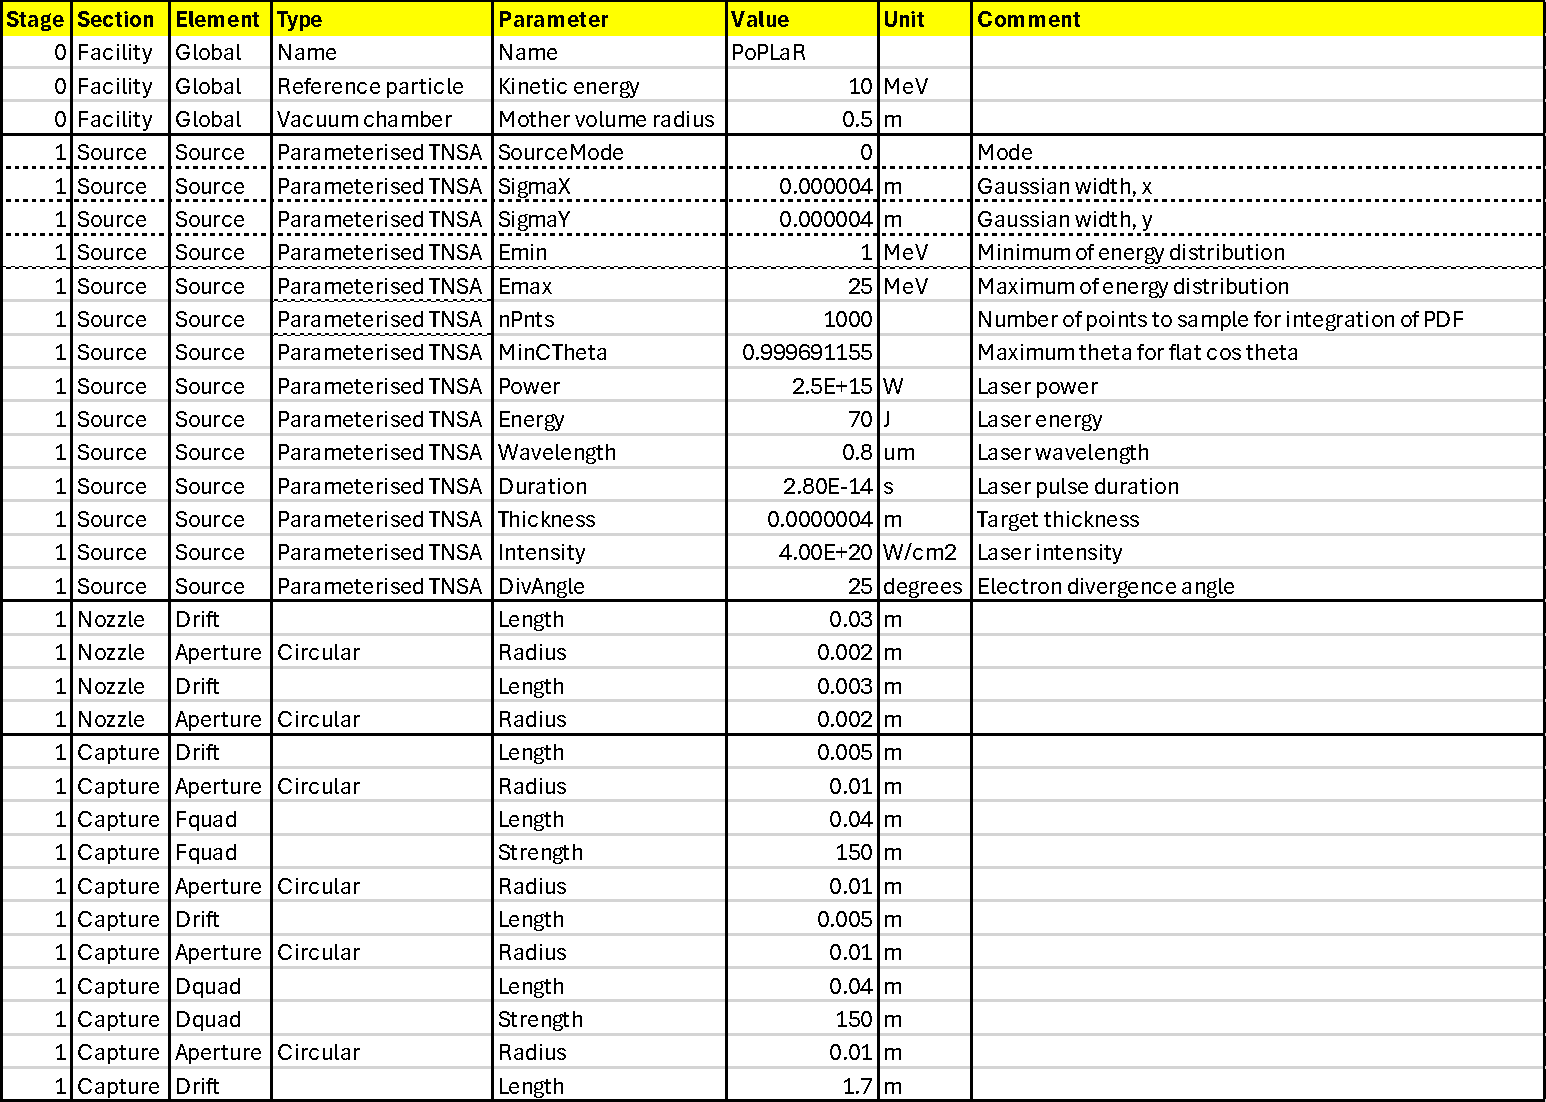
\includegraphics[width=\textwidth]{PoPLaR-BLspec.pdf}
  \end{center}
\end{table}

The beam line is built by reading the file sequentially from the top.
After the header fields, the first lines specify
the \texttt{Facility}, giving its \texttt{Name}, the kinetic energy of
the reference particle and radius of the ``mother volume''.
The mother volume is a cylinder around the beam line, a particle
hitting the boundary of the cylindrical volume is not propagated
further along the beam line.
The lines which follow specify each element of the beam line in turn,
grouping them by \texttt{Stage} and \texttt{Section} as requured.

\subsection{Scripts}

Scripts to perform common tasks are provided in
the \texttt{03-Scripts} directory.  
The scripts and the tasks they perform are;
\begin{description}
  \item{\texttt{runBeamSim.py -b <beamlinefile> -i <inputfile> -o <outputfile> -n <nEvts>}} \\
    uses the beam line specified in \texttt{<beamlinefile>} to
    generate \texttt{<nEvts>} and propagate them down the beam line.
    The output is written to \texttt{<outputfile>} in the format
    defined in the \texttt{BeamIO} class.
    If specified, \texttt{<inputfile>} is a \texttt{BeamIO} data
    file.
    In this case, beam transport starts from the most downstream
    element of the beam line defined in \texttt{<inputfile>}.
    Only one of \texttt{<beamlinefile>} and \texttt{<inputfile>} may
    be specified.
  \item{\texttt{readBeamSim.py -i <inputfile> -o <outputfile> -n <nEvts>}} \\
    reads \texttt{<nEvts>} events from the \texttt{BeamIO}-format
    data file \texttt{<inputfile>}.
    Two \texttt{PDF} files are written to \texttt{99-Scratch}.
    The first, \texttt{ParticleProgressionPlot.pdf}, contains plots of
    the transverse trace space coordinates of the particles at the
    exit of each beamm line element.
    The second, \texttt{ParticleLongiProgressionPlot.pdf}, contains
    plots of the longitudina trace space coordinates of the particles
    at the exit of each beamm line element.
    The option \texttt{-o <outputfile>} has not yet been
    implemented.
  \item{\texttt{plotBeam.py -i <inputfile> -n <nEvts> -o <outputfile> -l <startlocation> [-b <beamlinefile>]}} \\
    calculates the covariance matrix of the trace-space coordinates at
    the exit from each vbean-line element and uses these covariance
    matrices to calculate the RMS beam size and Twiss parameters.
    A \texttt{PDF} file, \texttt{BeamProgress.pdf}, showing the
    evolution of these quantities along the is written
    to \texttt{99-Scratch}.
    The calculations are performed on \texttt{<nEvts>} read
    from \texttt{<inputfile>}.
    If specified, a CSV file containing a summary of the beam
    evolution is written to \texttt{<outputfile>}.
    Optionally, if \texttt{-l} is specified, the beam line evolution
    will be plotted from from location \texttt{<startlocation>}.
    The option \texttt{-b <beamlinefile>} is retained in case early
    versions of \texttt{BeamIO}-format data files are to be read.
  \item{\texttt{plotextrapolatedBeam.py -i <inputfile> -n <nEvts> -o <outputfile> -l <startlocation> [-b <beamlinefile>]}} \\
    calculates the covariance matrix of the beam at
    location \texttt{<startlocation>} and then calculates the
    evolution of the covariance matrix and Twiss parameters using the
    beam-line element transfer matrices.
    The \texttt{PDF} file, \texttt{extrapolatedBeamProgress.pdf}, is
    created to contain plots of the beam evolution.
    If \texttt{<startlocation>} is not specified, the covariance
    matrix is calculated at the first element of the beam line and
    the propogation of the beam envelope starts at the beginning of
    the beam line.
    The meaning of the other switches are as
    for \texttt{plotBeam.py}.
  \item{\texttt{2BDSIM.py -i <inputfile> -o <outputfile> -l <start location> -n <nEvts>}} \\
    reads \texttt{<nEvts>} events from the \texttt{BeamIO}-format
    file \texttt{<inputfile>} and writes the ascii
    file \texttt{<outputfile>} in the format required by BDSIM.
    If specified, the BDSIM-format file is generated at
    location \texttt{<start location>}.
    If \texttt{<start location>} is not specified, the BDSIM-format is
    created with particles at the end of the beam line.
\end{description}
